%%%%%%%%%%%%%%%%%%%%%%%%%%%%%%%%%%%%%%%%%
% baposter Portrait Poster
% LaTeX Template
% Version 1.0 (15/5/13)
%
% Created by:
% Brian Amberg (baposter@brian-amberg.de)
%
% This template has been downloaded from:
% http://www.LaTeXTemplates.com
%
% License:
% CC BY-NC-SA 3.0 (http://creativecommons.org/licenses/by-nc-sa/3.0/)
%
%%%%%%%%%%%%%%%%%%%%%%%%%%%%%%%%%%%%%%%%%

%----------------------------------------------------------------------------
%	PACKAGES AND OTHER DOCUMENT CONFIGURATIONS
%----------------------------------------------------------------------------

\documentclass[a0paper,landscape,fontscale=0.395]{baposter}

\usepackage[font=small,labelfont=bf]{caption} % Required for specifying captions to tables and figures
\usepackage{booktabs} % Horizontal rules in tables
\usepackage{enumitem} % To change spacing in itemize and enumerate lists
\usepackage{multicol}
\usepackage{relsize} % Used for making text smaller in some places
\usepackage{amsfonts, amsmath, amsthm, amssymb} % For math fonts, symbols and environments
\usepackage{wrapfig} % Allows wrapping text around tables and figures
\usepackage[export]{adjustbox}% http://ctan.org/pkg/adjustbox
\usepackage{palatino} % Uncomment to use the Palatino font
\usepackage{graphicx} % Required for including images
\usepackage{color}
\usepackage{mathtools}

\graphicspath{{figures/}} % Directory in which figures are stored

\definecolor{bordercol}{RGB}{256,256,256} % Border color of content boxes
\definecolor{headercol1}{RGB}{51,0,111} % Background color for the header in the content boxes (left side)
\definecolor{headercol2}{RGB}{51,0,111} % Background color for the header in the content boxes (middle)
\definecolor{headerfontcol}{RGB}{256,256,256} % Text color for the header text in the content boxes
\definecolor{boxcolor}{RGB}{256,256,256} % Background color for the content in the content boxes

\newenvironment{Figure}
  {\par\medskip\noindent\minipage{\linewidth}}
  {\endminipage\par\medskip}

\DeclarePairedDelimiterX{\norm}[1]{\lVert}{\rVert}{#1}
\DeclareMathOperator{\Tr}{Tr}

\begin{document}

\begin{poster}{
    columns=5,
    grid=false,
    headerheight=0.1\textheight,
    borderColor=bordercol, % Border color of content boxes
    headerColorOne=headercol1, % Background color for the header in the content boxes (left side)
    headerColorTwo=headercol2, % Background color for the header in the content boxes (middle)
    headerFontColor=headerfontcol, % Text color for the header text in the content boxes
    boxColorOne=boxcolor, % Background color for the content in the content boxes
    headershape=roundedright, % Specify the rounded corner in the content box headers
    headerfont=\Large\sf\bf, % Font modifiers for the text in the content box headers
    textborder=rectangle,
    background=none,
    headerborder=open, % Change to closed for a line under the content box headers
    boxshade=plain
}
{}
%
%----------------------------------------------------------------------------
%	TITLE AND AUTHOR NAME
%----------------------------------------------------------------------------
%
{\sf\bf Multidimensional analysis and detection \\ of informative features in human brain white matter} % Poster title
{\vspace{0.5em} Adam Richie-Halford\textsuperscript{1}, Jason Yeatman\textsuperscript{2}, Noah Simon\textsuperscript{3} \& Ariel Rokem\textsuperscript{4} \hfill ISMRM 2021\hspace{0.5em}\null \\ % Author names
{\smaller 1. eScience Institute, 3. Dept. of Biostatistics, 4. Dept. of Psychology, University of Washington, 2. Stanford University \hfill Contact: richford@uw.edu \hspace{0.5em}\null}} % Author email addresses
{
\includegraphics[scale=0.12]{UWlogo.png}} % University/lab logo
\vspace{-10em}

%----------------------------------------------------------------------------
%	INTRODUCTION
%----------------------------------------------------------------------------

\headerbox{Introduction}{name=introduction,column=0,row=0}{
\noindent White matter structure is important to normal brain function. Diffusion tensor imaging (DTI) measures the white matter \emph{in vivo} by fitting a diffusion model in every voxel.

\vspace{0.5em}
\noindent\textbf{\underline{Challenge}: Make sense of the massive dimensionality of DTI data with comparatively few subjects in any given study.}
\vspace{0.5em}

\noindent One approach is to reduce the dimensionality of each tensor to scalars, e.g.~mean diffusivity (MD) or fractional anisotropy (FA).

\noindent Tractometry reduces the dimensionality of this data by quantifying diffusion metrics along tract profiles.

\begin{Figure}
    \centering
    \vspace{0.25cm}
    \rlap{
        \hspace{0.5em}
        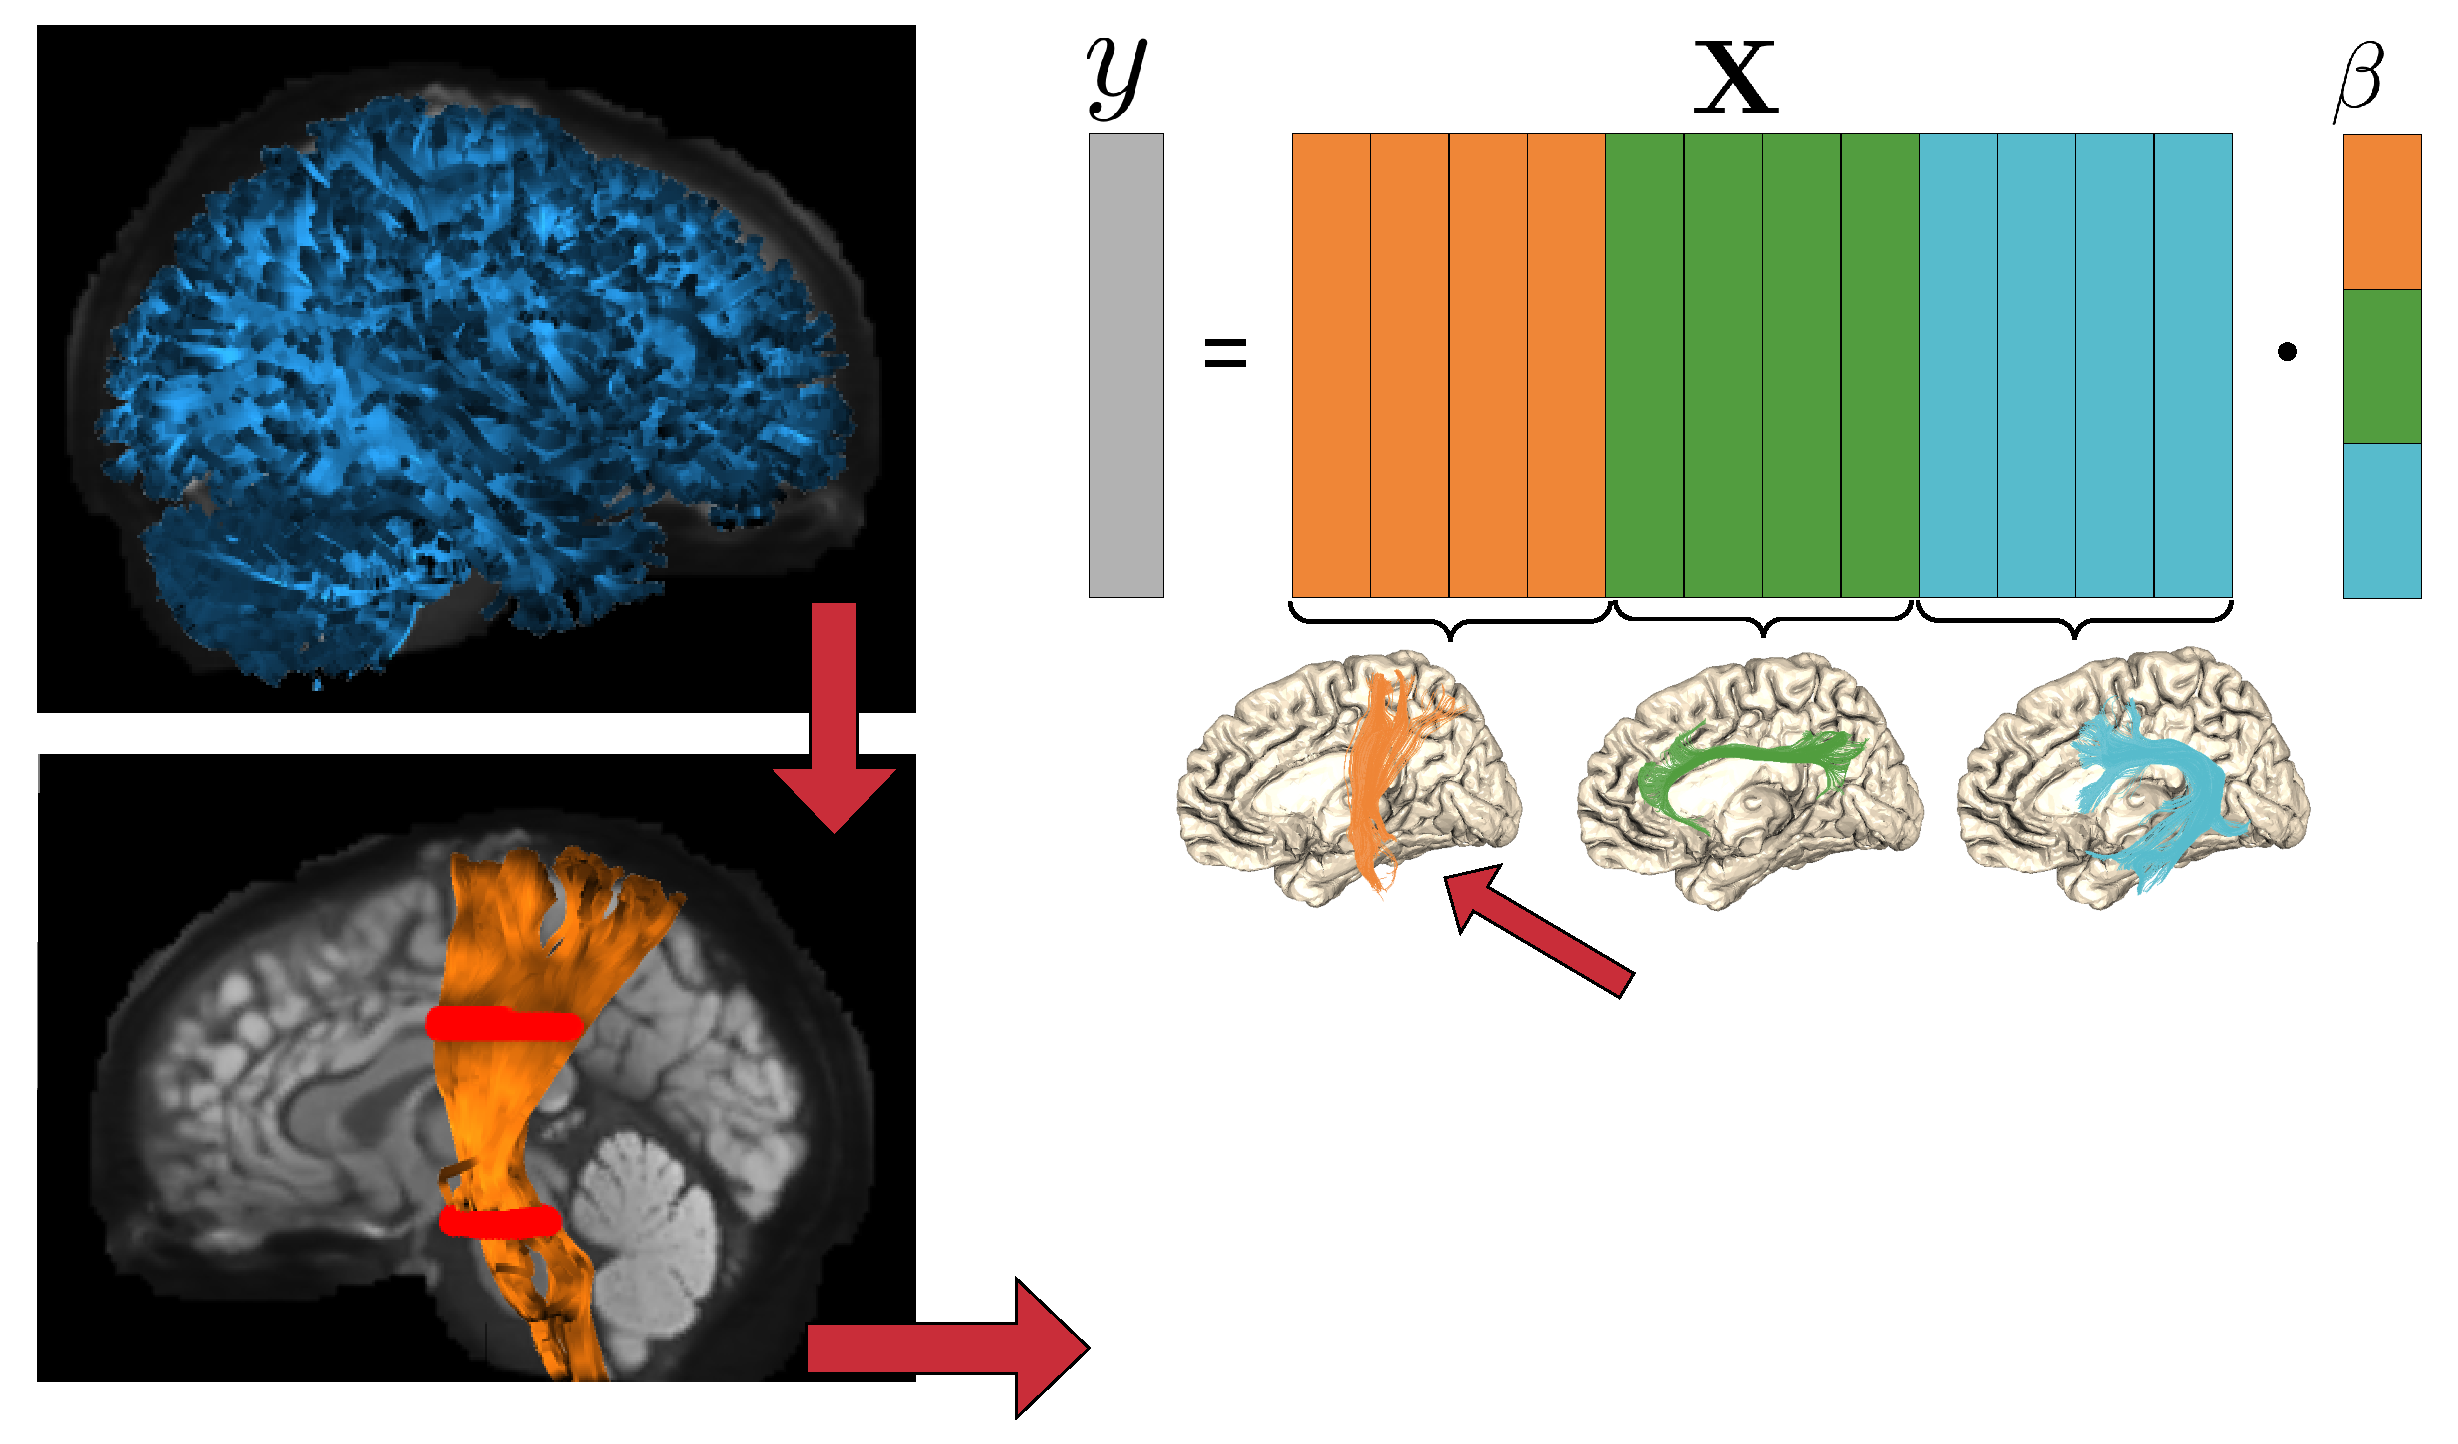
\includegraphics[width=0.98\linewidth]{methods-brains.pdf}
    }
    \vspace{-5cm}
    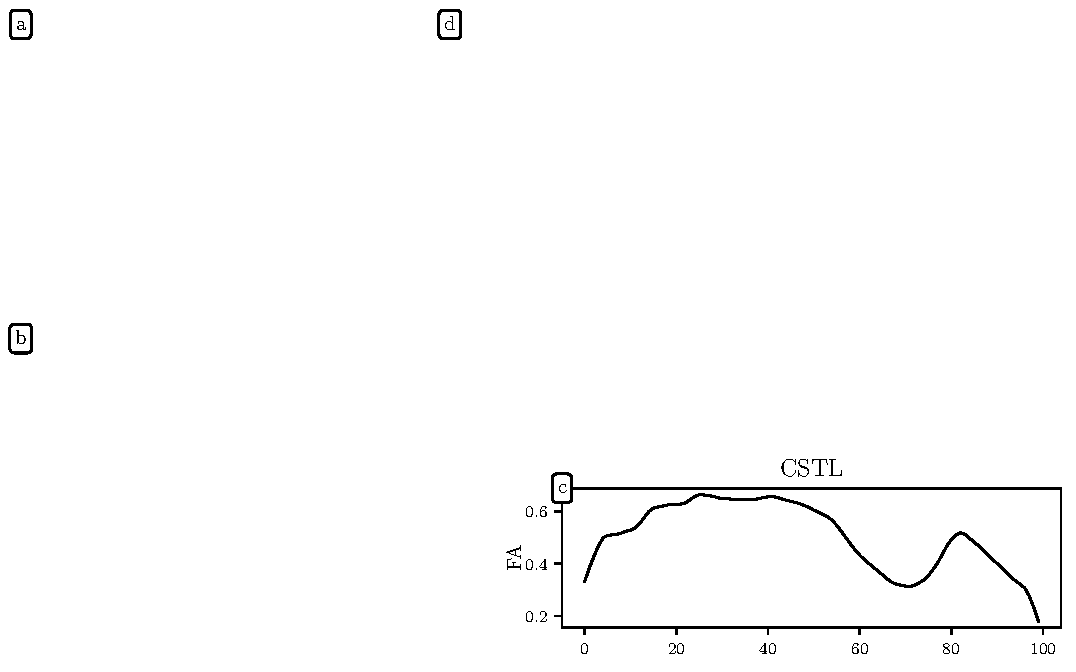
\includegraphics[width=0.98\linewidth]{method-quad.pdf}

    \captionof{figure}{{\bf Tractometry data flow}
        \label{fig:methods}
        {\bf (a)} Whole brain tractography generates streamlines approximating
        the trajectories of white matter connections.
        {\bf (b)} Tractometry classifies these streamlines into anatomical bundles.
        In this case, we show the left corticospinal tract (CSTL) over a mid-saggital
        anatomical slice.
        {\bf (c)} Tractometry further extracts \emph{bundle profiles}:
        quantifications of various diffusion metrics along the length of the
        fiber bundle. Here, we show one subject's fractional anisotropy (FA)
        profile for CSTL.
        {\bf (d)} the phenotypical target data and tractometric features can
        be organized into a linear model, $\hat{y} = \mathbf{X}
        \hat{\beta}$. The feature matrix $\mathbf{X}$ is color-coded
        to reveal a natural group structure: the left group
        contains $k$ features from the CSTL, the middle group
        contains $k$ features from the left cingulum cingulate,
        and the right group
        contains $k$ features from the left arcuate. The coefficients in
        $\hat{\beta}$ follow the same natural grouping.
    }
\end{Figure}
}

%----------------------------------------------------------------------------
%	CONCLUSION
%----------------------------------------------------------------------------

\headerbox{Conclusion}{name=conclusion,column=0,below=introduction,above=bottom}{

\begin{itemize}[nosep, leftmargin=*]
\item Novel method for analysis of dMRI tractometry data

    \begin{itemize}[nosep, leftmargin=*]
    \item Accurate prediction of phenotypic information
    \item Interpretable results and identification of important features
    \end{itemize}

\item Applicable to both localized and global phenomena
\item Packaged as open-source software called AFQ-Insight: \\ \texttt{https://github.com/richford/AFQ-Insight}

\item Integrates into broader AFQ software ecosystem:
    \begin{itemize}[nosep, leftmargin=*]
    \item pyAFQ: creates tractometry data from raw dMRI
    \item AFQ-Browser: visualization, analysis, and sharing
    \end{itemize}
\end{itemize}

}

%----------------------------------------------------------------------------
%	RESULTS 1
%----------------------------------------------------------------------------

\headerbox{Results: Classifying Patients with ALS}{name=results1,span=2,column=1,row=0}{ % To reduce this block to 1 column width, remove 'span=2'

\begin{itemize}[noitemsep, leftmargin=*]
    \item Previous study measured dMRI in patients with amyotrophic lateral sclerosis (ALS) (Sarica et al.~2017).
    \begin{itemize}[noitemsep, leftmargin=*]
        \item 24 ALS patients and 24 demographically matched controls
        \item Previous state of the art achieved 80\% accuracy using random forests and \emph{a priori} feature selection.
    \end{itemize}
    \item Our method outperforms previous results, with a cross-validated accuracy of 83\% and an AUC-ROC of 0.88.
    \item Moreover, it automatically identifies the corticospinal tract (CST) as the critical feature for differentiating patients with ALS from controls
    \item Thus, well-known features of the disease can be recovered through an automated, data-driven approach.
\end{itemize}
\begin{Figure}
    \centering
    \vspace{4cm}
    \rlap{
        \hspace{1.75cm}
        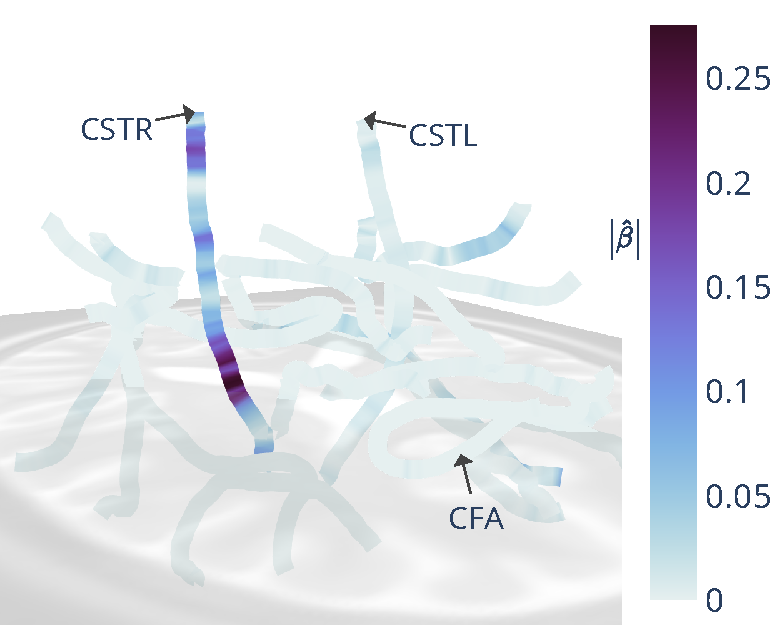
\includegraphics[width=0.25\linewidth]{als_coefs.pdf}
    }
    \vspace{-7.5cm}
    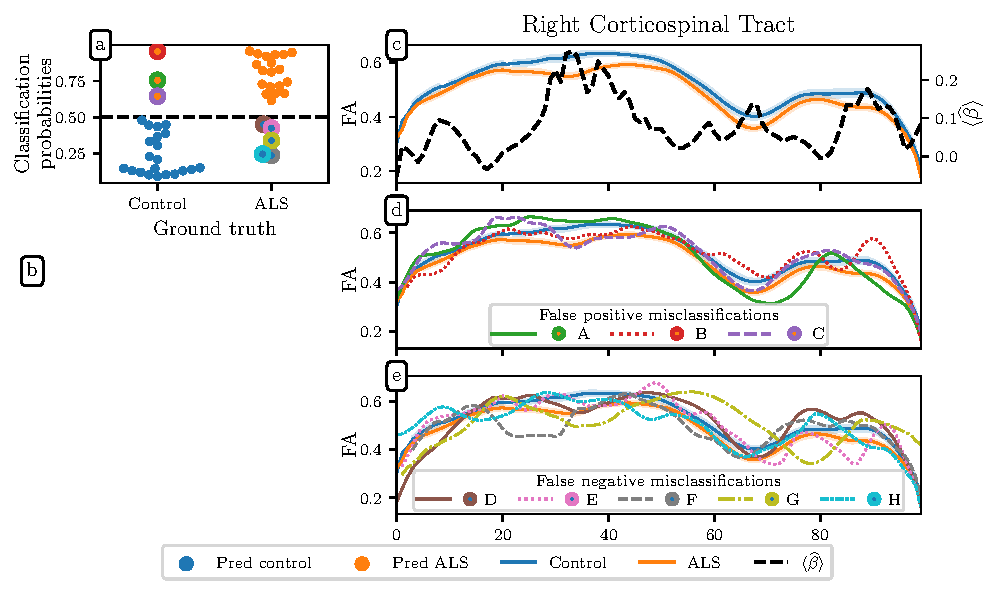
\includegraphics[width=0.85\linewidth]{als_results.pdf}
    \captionof{figure}{
        {\bf SGL accurately and interpretably predicts ALS diagnosis.}
        {\bf (a)} Classification probabilities for ALS diagnosis, with
        controls on the left, patients on the right, predicted controls in
        blue, and predicted patients in orange. That is, orange dots on the left
        represent false positives, while blue dots on the right represent
        false negatives. We achieve 83\% accuracy with an
        ROC AUC of 0.88.
        {\bf (b)} SGL coefficients are presented on the core fibers of major
        fiber bundles. They exhibit high group sparsity and are concentrated
        in the FA of the CST. The brain is oriented with the right hemisphere
        in the foreground and anterior to the right of the page. The CSTL,
        CSTR, and CFA bundles are indicated for orientation.
        {\bf (c)} SGL identifies three portions of the CST as important,
        where $\hat{\beta}$ (dashed line, right axis) has large values. These
        are centered around nodes 30, 65, and 90, corresponding to locations
        of substantial differences in FA between the ALS and control groups
        (shaded areas indicates standard error of the mean).
        {\bf (d)} Bundle profiles for false positive classifications. Line
        colors correspond to the marker edge color in the top left plot.
        These individuals have reduced FA in the CST portions which SGL
        identified as important. Their misclassification is coherent with the
        feature importance and the group differences in FA.
        {\bf (e)} Individual bundle profiles for false negative
        classifications. These individuals have bundle profiles which
        oscillate between the group means.
    }
\end{Figure}
}

%----------------------------------------------------------------------------
%	RESULTS 2
%----------------------------------------------------------------------------

\headerbox{Results: Predicting ``Brain Age''}{name=results2,span=2,column=3,row=0}{ % To reduce this block to 1 column width, remove 'span=2'

\begin{itemize}[noitemsep, leftmargin=*]
    \item In a regression setting, SGL can predict ``brain age'' in three previous studies.
    \begin{itemize}[noitemsep, leftmargin=*]
        \item Weston-Havens (WH): 76 subjects with ages 6-50 (Yeatman et al.~2014)
        \item Healthy Brain Network (HBN): 978 subjects with ages 5-21 (Alexander et al.~2017)
        \item Cam-CAN: 640 subjects with ages 18-88 (Shafto et al.~2014)
    \end{itemize}
    \item We predict subjects' chronological age with competitive performance (see Figure 3).
    \item Older subjects have higher residual variance, reflecting the automatically-chosen log-transformation and implying that brain age becomes more difficult to predict as we age chronologically.
    \item In contrast to the ALS classification case, brain age feature importance is dense and non-localized.
\end{itemize}

\begin{Figure}
    \centering
    \vspace{3.5cm}
    \rlap{
        \hspace{2cm}
        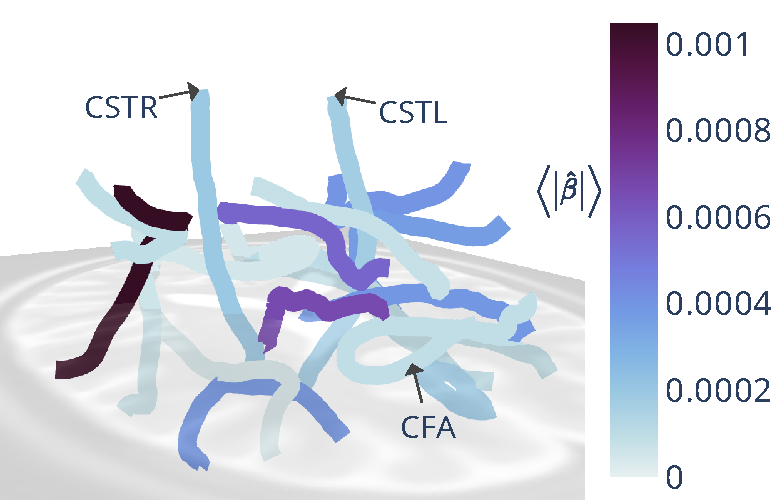
\includegraphics[width=0.25\linewidth]{wh_coefs.pdf}
        \hspace{0.25em}
        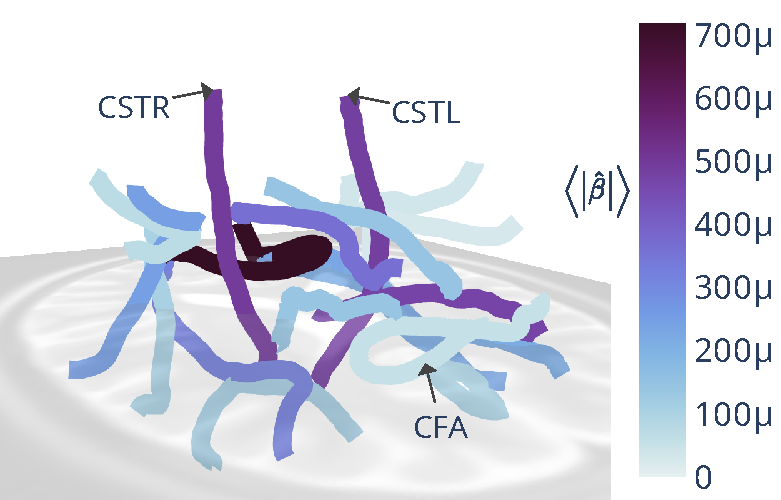
\includegraphics[width=0.25\linewidth]{hbn_coefs.pdf}
        \hspace{0.25em}
        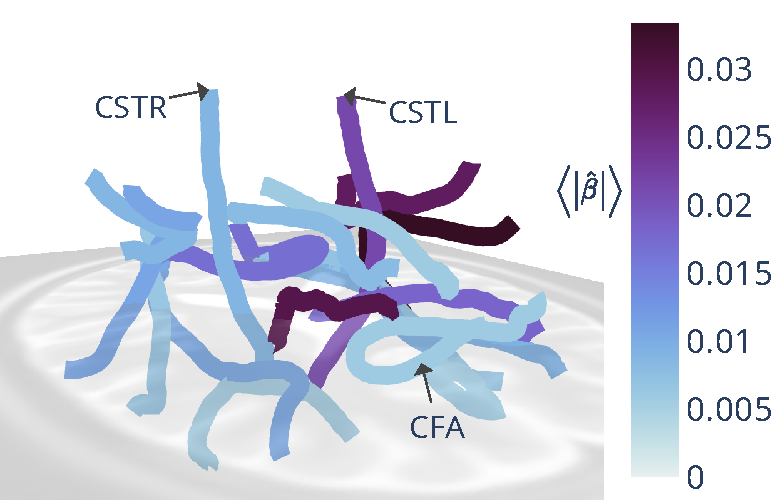
\includegraphics[width=0.25\linewidth]{camcan_coefs.pdf}
    }
    \vspace{-7cm}
    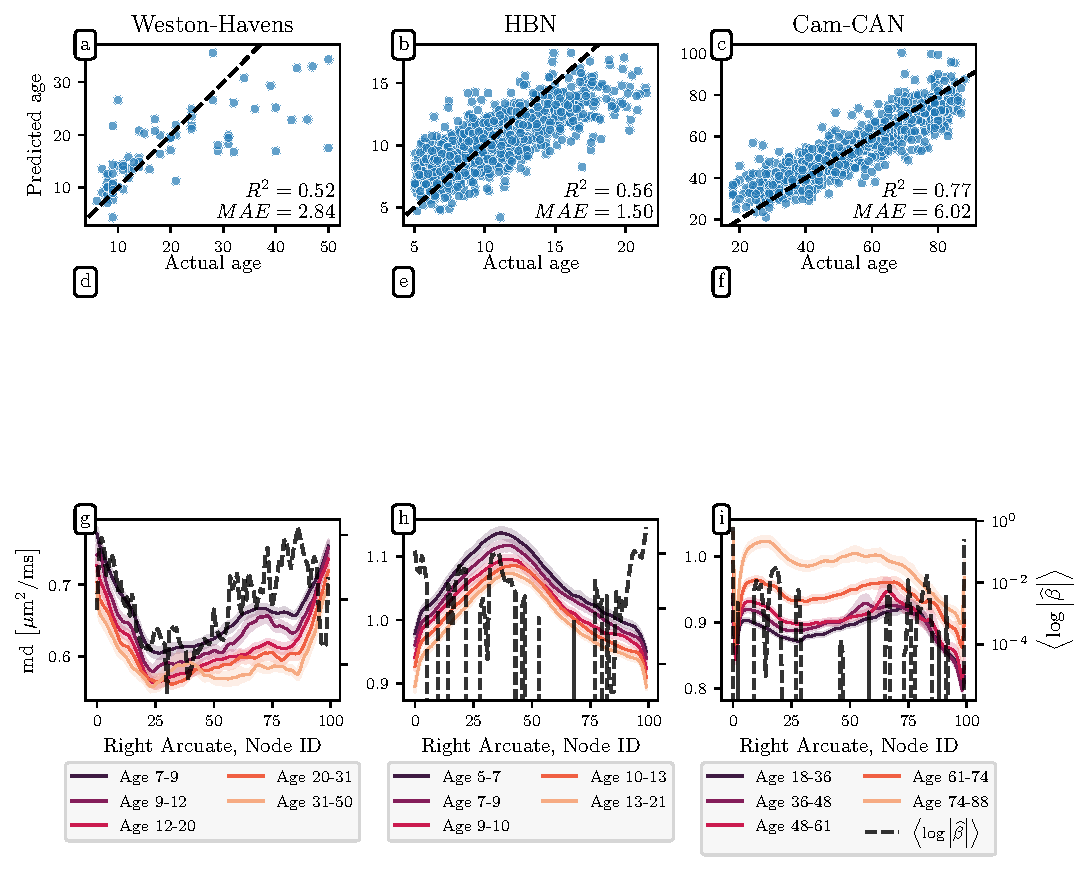
\includegraphics[width=0.85\linewidth]{regression_scatter.pdf}
    \captionof{figure}{
        {\bf Predicting age with tractometry and SGL.}
        {\bf (top)} The predicted age vs. true age of each individual from the test
        splits (i.e., when each subject's data was held out in fitting the
        model) for the {\bf (a)} WH, {\bf (b)} HBN, and {\bf (c)} Cam-CAN
        datasets; an accurate prediction falls close to the $y=x$ line
        (dashed). The mean absolute error (MAE) and coefficient of
        determination $R^2$ are presented in the lower right of each scatter
        plot.
        {\bf (middle)} Feature importance for predicting age from tractometry in
        the {\bf (d)} WH, {\bf (e)} HBN, and {\bf (f)} Cam-CAN datasets.
        The orientation of the
        brain is that same as in Figure 2b, however because
        the coefficients exhibit high global sparsity (as opposed to group
        sparsity), we plot the mean of the absolute value of $\hat{\beta}$
        for each bundle on the core fiber. The global distrubution of the
        $\hat{\beta}$ coefficients reflects the fact that aging is not
        confined to a single white matter bundle.
        {\bf (bottom)} Age quintile bundle profiles for the {\bf (g)} WH,
        {\bf (h)} HBN, and {\bf (i)} Cam-CAN datasets.
    }
\end{Figure}
}

%----------------------------------------------------------------------------
%	METHODS
%----------------------------------------------------------------------------

\headerbox{Methods}{name=methods,column=1,span=4,below=results2}{

\begin{multicols}{2}
\begingroup
We use AFQ to generate tractometry data as input to our model and then fit a linear model to the data,
\begin{equation*}
    y = \mathbf{X} \cdot \beta,
\end{equation*}
\vspace{-2.25em}
where
\begin{align*}
    y &\coloneqq \text{phenotype} \; (n_\text{subjects} \times 1), \\
    \mathbf{X} &\coloneqq \text{tractometry data} \; (n_\text{subjects} \times n_\text{features}), \\
    \beta &\coloneqq \text{regression coefficients} \; (n_\text{features} \times 1).
\end{align*}
The feature matrix, $\mathbf{X}$, has inherent group structure, containing groups for each diffusion metric and each fiber bundle.
The high dimensionality of the data ($n_\text{features} \sim \mathcal{O}(10^4)$) requires regularization to avoid overfitting, via the Sparse Group Lasso (SGL),
\vspace{-0.5em}
\begin{equation*}
    \widehat{\beta} = \min_\beta \Biggl\{
        \underbrace{
            \vphantom{(1 - \alpha) \lambda \displaystyle \sum_\ell \sqrt{p_\ell} \norm{\beta^{(\ell)}}_2}
            \norm{\widehat{y} - \mathbf{X} \cdot \beta}_2^2
        }_{\text{Linear regression}}
        + \underbrace{
            (1 - \alpha) \lambda \displaystyle \sum_\ell \sqrt{p_\ell} \norm{\beta^{(\ell)}}_2
        }_{\text{Group Lasso Penalty}}
        + \underbrace{
            \vphantom{(1 - \alpha) \lambda \displaystyle \sum_\ell \sqrt{p_\ell} \norm{\beta^{(\ell)}}_2}
            \alpha \lambda \norm{\beta}_1
        }_{\text{Lasso Penalty}}
    \Biggl\}
\end{equation*}
SGL enforces sparsity at both the \textbf{inter}-group level (using $\alpha =
0$) and \textbf{intra}-group level (using $\alpha = 1$). The hyperparameters
$\lambda, \alpha$ are optimized through nested $k$-fold
cross-validation.
\endgroup
\end{multicols}
}

%----------------------------------------------------------------------------
%   REFERENCES
%----------------------------------------------------------------------------

\headerbox{References}{name=references,column=0,span=4,below=methods,above=bottom}{

\begin{multicols}{2}
\smaller \smaller % Reduce the font size in this block
\renewcommand{\section}[2]{\vskip 0.05em} % Get rid of the default "References" section title
\nocite{*} % Insert publications even if they are not cited in the poster

\bibliographystyle{unsrt}
\bibliography{poster}
\end{multicols}
}

%----------------------------------------------------------------------------
%	ACKNOWLEDGMENTS
%----------------------------------------------------------------------------

\headerbox{Acknowledgments}{name=acknowledgments,column=4,span=1,below=methods,above=bottom}{

\begin{multicols}{2}
\smaller % Reduce the font size in this block

\includegraphics[height=0.8cm]{nimh-logo.png}


\includegraphics[height=0.75cm]{eSciencelogo.png}


\includegraphics[height=0.5cm]{logo_gcp_horizontal_rgb.png}

\hspace{0.5em} 
\includegraphics[height=0.88cm]{SloanLogo.png}

\hspace{0.5em} 
\includegraphics[height=0.88cm]{MooreFdn.png}


\end{multicols}
}

\end{poster}

\end{document}
